\documentclass[3p, 12pt]{elsarticle} %3p

\usepackage{amsmath}
\usepackage{amsfonts} %potrzebne do \mathbb{S}

\usepackage{here}


\usepackage{caption}
\usepackage{subcaption}

\usepackage{color}
\newcommand{\norm}[1]{\left\lVert#1\right\rVert}
\def\spe{\mathbf{Spec}}

\usepackage{graphicx}

\usepackage{soul}           %package for highlight
\newcommand{\noop}[1]{}
\newtheorem{problem}{Problem}

\usepackage{lineno,hyperref}
\modulolinenumbers[5]

\journal{Mechanical Systems and Signal Processing}

%%%%%%%%%%%%%%%%%%%%%%%
%% Elsevier bibliography styles
%%%%%%%%%%%%%%%%%%%%%%%
%% To change the style, put a % in front of the second line of the current style and
%% remove the % from the second line of the style you would like to use.
%%%%%%%%%%%%%%%%%%%%%%%

%% Numbered
%\bibliographystyle{model1-num-names}

%% Numbered without titles
%\bibliographystyle{model1a-num-names}

%% Harvard
%\bibliographystyle{model2-names.bst}\biboptions{authoryear}

%% Vancouver numbered
%\usepackage{numcompress}\bibliographystyle{model3-num-names}

%% Vancouver name/year
%\usepackage{numcompress}\bibliographystyle{model4-names}\biboptions{authoryear}

%% APA style
%\bibliographystyle{model5-names}\biboptions{authoryear}

%% AMA style
%\usepackage{numcompress}\bibliographystyle{model6-num-names}

%% `Elsevier LaTeX' style
%\bibliographystyle{abbrvnat}%\biboptions{sort&compress}
\bibliographystyle{elsarticle-num}\biboptions{sort&compress}
%%%%%%%%%%%%%%%%%%%%%%%

\begin{document}

\begin{frontmatter}

% \title{Compound interdimensional approach using nonnegative matrix factorization with spatial denoising for identification of impulsive damage component\par 
% \title{Impulsive source separation using NMF factorization of spatially denoised bi-frequency map\par 
\title{Impulsive source separation using combination of Nonnegative Matrix Factorization of bi-frequency map, spatial denoising and Monte Carlo simulation}
% jerome mssp separacja a ekstrakcja

%% Group authors per affiliation:
\author[label1]{Jacek Wodecki \corref{cor1}}
\author[label3]{Anna Michalak}
\cortext[cor1]{Corresponding author, jacek.wodecki@pwr.edu.pl}
\author[label1]{Rados{\l}aw Zimroz}
\author[label2]{Tomasz Barszcz}
\author[label3]{Agnieszka Wy{\l}oma{\'n}ska}

\address[label1]{Faculty of Geoengineering, Mining and Geology, Wroclaw University of Science and Technology, Na Grobli 15, 50-421 Wroclaw, Poland
\\\{jacek.wodecki, radoslaw.zimroz\}@pwr.edu.pl\\}
\address[label2]{AGH University of Science and Technology, Krakow, Poland
\\ tbarszcz@agh.edu.pl\\}
\address[label3]{KGHM Cuprum Ltd, Research and Development Centre, Sikorskiego 2-8, 53-659 Wroclaw, Poland
 \{amichalak, awylomanska\}@cuprum.wroc.pl\\}

\begin{abstract}

In this paper, authors present the original procedure for local damage detection in rolling bearings based on vibration data. The aim is to obtain envelope spectrum (ES) of the signal component related to damage, that is clear and easy to interpret. The method is especially aimed at cases, when multiple cyclic impulsive components are present and interfere with each other, which makes ES of such signal very difficult to evaluate. In order to deal with such situation properly, authors propose to choose Cyclic Spectral Coherence (CSC) map as a two-dimensional data representation that will be the basis for the analysis. Nonnegative Matrix Factorization (NMF) is used to analyze such map in two ways: first, it helps to initially separate cyclic components by producing a set of filters for input vibration data, and second, to identify proper damage-related frequency components in envelope spectrum. In addition, an intermediate step of spatial denoising allows enhancing the properties of CSC map. Finally, Monte Carlo simulation improves statistical significance of the result and increases robustness by reducing the impact of random initialization effects. The method has been evaluated using real-life vibration data measured on rolling bearing operating in the industrial gas compressor.
\end{abstract}

\begin{keyword}
vibration, damage detection, bearings, cyclostationarity, nonnegative matrix factorization, spatial denoising, Monte Carlo simulation, separation
\end{keyword}

\end{frontmatter}

\linenumbers

\section{Introduction}
Local damage detection is a very popular topic in condition monitoring of rotating machines. There are plenty of powerful solutions that are able to detect damage in rolling element bearings or gearboxes, even if impulsive signature related to damage is hidden in measured vibration \cite{samuel2005review,randall2011rolling}. Most of methods are based on detection of impulsive character of so-called signal of interest (SOI) \cite{antoni2006spectral,wodecki2018optimal} or cyclic/periodic nature of SOI \cite{cioch2013finding}. Although the effectiveness of the mentioned method is very high, there are still some challenges in this area. One of them is time-varying operating conditions, in such a case both amplitude of impulses as well as cycle length might be load/speed dependent \cite{gryllias2018application}.

Another challenge is related to presence of impulsive background noise \cite{wylomanska2017application,wylomanska2016impulsive,zak2014application, antoni2016infogram,puchalski2017stable,yu2013new}. It could be real impulsive noise, or other source of vibration that produce impulsive signal, other damage located on another component \cite{kruczek2017cyclic}, process that is performed by machine like crushing \cite{wylomanska2016impulsive} or cyclic operation of valves \cite{antoni2002effective,barszcz2013bearings}, or tools \cite{cocconcelli2012algorithm}

In this paper, we will consider a specific signal that contains two impulsive sources: one is related to mentioned process (cyclic operation of the compressor), while the second one is related to relatively small energy impulsive contribution from faulty bearings located in this compressor. Raw vibration data reveals cyclic impulses related to the process of gas compression, while damage signature is hidden. 

This and similar signals have been already studied for impulsive component extraction in the presence of more than one impulsive components, with various quality of results. NMF as of itself provided acceptable results for similar simulated signal, however in that case spectrogram worked well enough as a base data representation \cite{wodecki2017novel}. Cyclostationary approach has also been proposed for this exact data, although while presented result was relatively good quality (some level of noise floor in envelope spectrum was still remaining though), algorithm required decision-making input from the user, which is not favouring in terms of automation and robustness \cite{barszcz2013bearings}. Similar simulated data containing multiple impulsive components has been also analyzed using double protrugram \cite{kruczek2017modified}, however this method also requires the user input for certain parameters, and only provides IFB selector for signal filtration, which carries over the noise imperfections.

Even if cyclostationary analysis if used, detection of damage in presence of high energy impulsive contamination is challenging. Hence, authors propose a multi-stage methodology that uses bi-frequency map as a base data representation for the analysis. However, as mentioned above, due to multiple sources of cyclic signals, CSC map is hard to analyze. In order to extract sources related to damage (and ignore source related to process), the content of such map is analyzed using Nonnegative Matrix Factorization (NMF). To enhance properties of CSC map, the intermediate step of spatial denoising is introduced. Finally, to deal with the uncertainty of stochastic aspect of analysis, Monte Carlo simulation allows obtaining the final diagnostic feature that is characterized by enhanced information clarity.

The main idea behind presented methodology assumes extraction of partial information from a two-dimensional representation of vibration data, namely CSC map. In order to achieve that goal, NMF is used. It has been shown that NMF is a powerful tool in data analysis and clustering \cite{cichocki2009nonnegative, wang2013nonnegative,lee1999learning, he2011symmetric}. In presented approach NMF is used for clustering of spectral content for each $\alpha$ frequency, similarly to the approach of clustering spectra for each time point in the spectrogram matrix \cite{wodecki2017local}.
Typical applications of NMF are focused on using information contained in only one of the factors produced by given NMF algorithm, while in presented method authors propose to analyze both output matrices in sequence. First, \emph{base matrix} is used for preliminary extraction of SOI, and after that \emph{encoding matrix} allows to precisely identify diagnostic information.

After extraction of damage-related part of CSC map, it is integrated to a 1D vector that might be considered as equivalent to envelope spectrum \cite{randall2011rolling}.
It should be noted that integration of original CSC map (without proposed processing) has complicated structure and identification of fault frequencies is difficult. Application of proposed procedure allows obtaining a very clear picture of envelope spectrum for inner race fault.

\section{Object of interest}

The studied machine is a gas compressor of a type Dresser-Rand C-VIP, that has been already studied by Barszcz et al. \cite{barszcz2013bearings}. The key issue is that vibration signals generated by the compressor contain a number of external disturbances, the most influential being the piston-related and valve-related ones. It has been discovered that the analyzed signal has been recorded when the bearing inner ring has been severely defected in one of the main shaft bearings. Figure~\ref{fig:raw} presents the time series of raw vibration data. Details including the SOI parameters are presented in Table~\ref{tab:tab1}. 

\begin{table}[ht!]
    \centering
    \caption{Machine-related frequencies}
    \begin{tabular}{|l|l|}
    \hline
         \textbf{Parameter} & \textbf{Frequency [Hz]} \\ \hline
         Sampling frequency & 24000 \\ \hline
         Shaft speed & 12.35 \\ \hline
         BPFI & 127.9 \\ 
    \hline
    \end{tabular}
    \label{tab:tab1}
\end{table}

\begin{figure}[ht!]
\centering
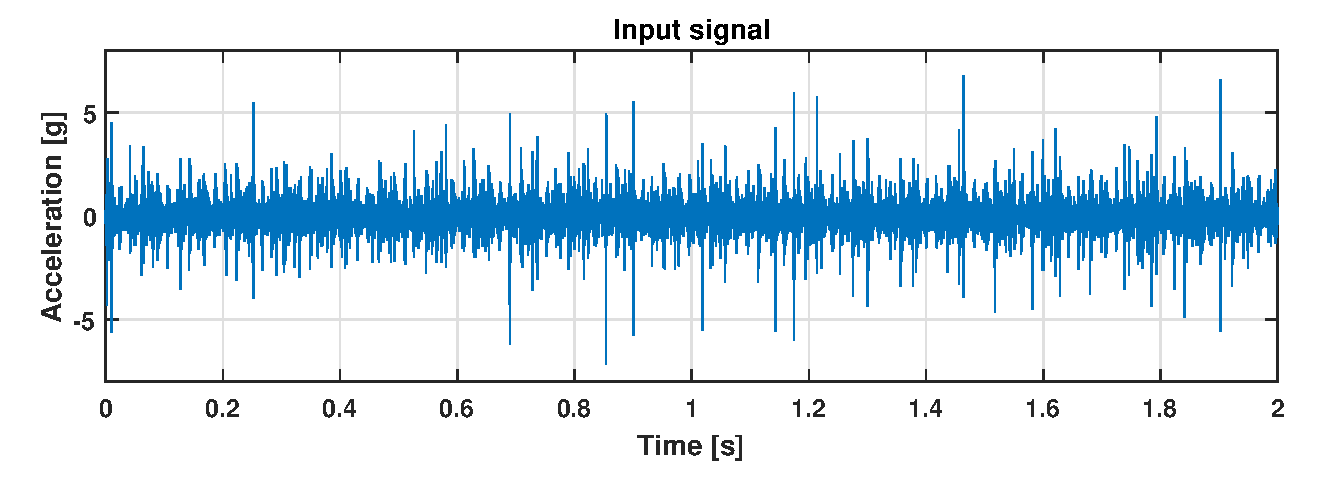
\includegraphics[width=0.7\textwidth]{wykresy/raw}
\caption{Raw vibration data}
\label{fig:raw}
\end{figure}

\begin{figure}[ht!]
\centering
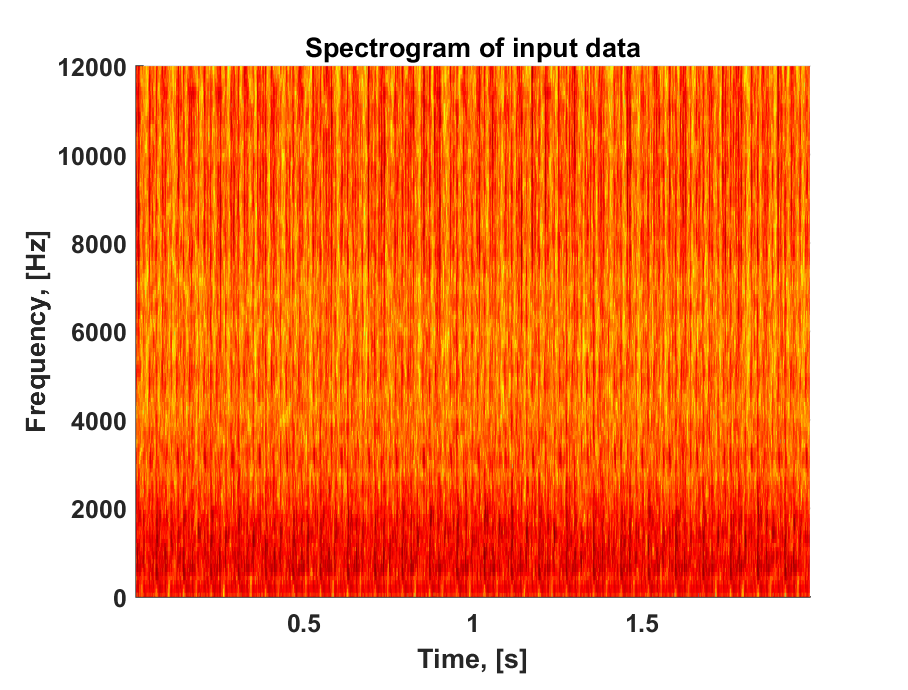
\includegraphics[width=0.7\textwidth]{wykresy/spec}
\caption{Time-frequency representation of vibration data}
\label{fig:spec}
\end{figure}

Impulses at the rate of approximately 12.35 Hz are observable. They reveal themselves directly on the DFT spectrum, dominating its low-frequency part (up to about 3 kHz), while the further part of the spectrum appears to be a noise-like behavior. Since the 12.35~Hz is the rotational speed, it is obvious that the main impulsive component is piston and valve-related. Bearing fault related impacts are not detectable on the spectrum.

Figure \ref{fig:spec} presents the spectrogram of input data. While shaft-related cyclic behavior is noticeable, SOI-related periodicity is not detectable based on such representation, which is the reason of employing different domain.

\section{Methodology}\label{met}

\begin{figure}[ht!]
\centering
\includegraphics[width=0.6\textwidth]{wykresy/block4}
\caption{Flowchart of proposed procedure}
\label{fig:block}
\end{figure}

In this section, authors present the details of the presented method. The main idea is focused on utilizing all the information that the factorization algorithm can provide for such problem. Typically when NMF is used, authors of proposed methods are only interested in the information held by one of the output matrices. One of the typical examples is time-frequency map analysis \cite{wodecki2017local}, where authors use \emph{encoding matrix} to classify spectra vectors in the time domain, allowing to extract impulses from vibration data. While the method is effective, it is important to note that the \emph{base matrix} remains unused, leaving behind the information that can still be of some value. Based on this idea, authors of presented paper propose to utilize the information from both output matrices in a sequential manner. 

Since the input vibration signal has a relatively complex structure in terms of the presence of cyclic components, instead of time-frequency representation authors decided to use the bi-frequency representation called Cyclic Spectral Coherence (CSC) as a basis for the analysis (see section~\ref{cscs}). In the first stage of processing, CSC map is firstly factorized with NMF algorithm, and the base matrix is used as a set of filters in the carrier frequency domain. Then, the input signal is filtered through a selected filter, which results in significant improvement of the signal in terms of SOI detectability \cite{wodecki2017novel}. 

In the second stage of processing obtained signal is spatially denoised in the bi-frequency domain. In order to achieve that, every vector of full modulating frequency range within a single carrier frequency bin is modeled with decaying exponential function (see section~\ref{denoise}). This way it is possible to construct a spatial noise model in the form of a matrix with the same dimensions as CSC matrix. After subtracting noise model matrix from CSC map, the latter becomes more clear and visibility of damage-related frequency components is improved.

In the third stage, denoised CSC map is again factorized with NMF algorithm within the iterations of Monte Carlo (MC) simulation. In each iteration damage-related envelope spectrum is extracted, and after averaging final form of envelope spectrum is obtained (see section \ref{mcmc}).

\subsection{Cyclic Spectral Coherence}\label{cscs}

In rotating machinery signals one can see different modulating frequencies for each carrier frequency. It is the reason why there is a need to apply methods based on the bi-frequency representation of given signal. In this paper, we propose to use the methodology proposed by Antoni in 2007, \cite{antoni2007cyclic}, who \textcolor{red}{first demonstrated the capacity of spectral coherence (SC) for bearing diagnostics and for machine signal analysis in general}. First, we introduce the cyclic power spectrum (CPS). The CPS $S_X(f;\alpha)$ for cyclostationary signal $\mathbf{x}$ is defined as follows:

\begin{equation}
\label{eq:CPS}
S_X(f;\alpha)=\lim_{L\to \infty} \frac{1}{L}\mathbb{E} \left(\mathcal{F}_{\mathbf{x},L} \left(f+\frac{\alpha}{2}\right)\overline{\mathcal{F}_{\mathbf{x},L}\left(f-\frac{\alpha}{2}\right)}\right),
\end{equation}
where $\mathcal{F}_{\mathbf{x},L}(f)$ is a Fourier transform of given signal $\mathbf{x}$ calculated on interval of length $L$. It is worth to mention, the CPS is interpreted as the dependence of the spectral components being apart by given modulating frequency $\alpha$ for carrier frequency $f$. For the cyclostationary signal we expect to have $\left|S_X(f;\alpha)\right|>0$ for modulation frequency $\alpha\neq 0$. The SC is defined as follows, ~\cite{antoni2007cyclic}:

\begin{equation}
\label{eq:SC}
\left|\gamma_X(f;\alpha)\right|^{2}=\frac { \left|S_X(f;\alpha)\right|^2 }{ S_X(f+\frac{\alpha}{2};0)S_X(f-\frac{\alpha}{2};0)}.
\end{equation}

As one can see, the statistic defined above is normalized. Therefore, one can interpret SC as the spectral cyclic autocorrelation. \textcolor{red}{In case $\left|\gamma_X(f;\alpha)\right|^{2}>0.05$  then we assume the signal exhibits the cyclostationarity property at carrier frequency f with modulation period equal to $T=1/\alpha$. In this case the threshold of $0.05$ is set to differentiate between ever-present noise of relatively low non-zero values across the entire map, and actual significant values at particular informative frequencies.}
The estimator of SC can be calculated by using the formula of an estimator for CPS. It is given by the following formula:

\begin{equation}
\left|\hat{\gamma}_X(f;\alpha)\right|^{2}=\frac{ \left|\hat{S}_X(f;\alpha)\right|^2 
}{\hat{S}_X(f+\frac{\alpha}{2};0)\hat{S}_X(f-\frac{\alpha}{2};0)},
\end{equation} 
where $\hat{S}_X(f;\alpha)$ is an estimator of the CPS defined as:

\begin{equation}
\hat{S}_X^{(L)}(f;\alpha)=\frac{1}{KF_S\norm{w}^2}\sum_{k=0}^{K-1}X^{(k)}_{Nw}\left( f+\frac{\alpha}{2}\right)X^{(k)}_{Nw}\left( f-\frac{\alpha}{2}\right)^*
\end{equation} 
where

\begin{equation}
X^{(k)}_{Nw}\left( f\pm\frac{\alpha}{2}\right)=\sum_{n=kR}^{kR+N_w-1}w_k[n]x[n]e^{\pm j\pi\alpha n/F_s}e^{-j2\pi fn/F_s}
\end{equation} 
is the discrete Fourier transform (DFT) of the $k^{th}$ weighted sequence $w_k[n]x[n]e^{\pm j\pi\alpha n/F_s}, K=\lfloor (L-N_w)/R\rfloor+1$ (where $\lfloor x \rfloor$ stands for the greatest integer smaller than or equal to x) is the total number of averaged segments, and $\norm{w}$ stands for the window root-mean-squared (RMS) value. 

\subsection{NMF}
Thanks to inherent clustering properties of NMF-type algorithms they can be used to aggregate different types of behavior within the analyzed matrix into separate classes. The presented methodology uses classic NMF with Euclidean objective function and multiplicative update rule.

Let $\bf{V}_{n\times m}$ denote input matrix containing only non-negative elements. For such data, Lee and Seung proposed a factorization into two components \cite{lee2001algorithms}:

\begin{equation}\label{V1} 
    {\bf V}_{n\times m}\simeq
    {\bf W}_{n\times r}{\bf H}_{r\times m}. 
\end{equation} 

where ${\bf W}$ and ${\bf H}$ also have to be non-negative, such as:
\begin{align*}
    &v_{ij}\ge0,~~w_{ik}\ge 0,~~ h_{kj}\ge 0,\\
    &~~i=1, \dots, n; ~j=1,\dots, m;
                ~~k=1,\dots,r.
\end{align*}

The parameter $r$ is supposed to satisfy the inequality: \mbox{$r~<= min(n,m)$},~ typically \mbox{$r~<<min(n,m)$}, where $<<$ stands for \emph{significantly smaller}. From now on, the parameter \emph{r} will denote the expected number of components in the signal.

Data matrix \textbf{V} contains in its columns \textit{m} 'objects', while each 'object' is characterized by \textit{n} variables. Equation (\ref{V1}) informs the reader that the original data matrix \textbf{V} is approximated by the product of real-valued lower rank matrices: \emph{base matrix} ${\bf W}_{n\times r}$ and \emph{encoding matrix} ${\bf H}_{r\times m}$  which have jointly less elements than ${\bf V}$, i.e. the following inequality holds:

\begin{equation}\label{r1}
    (n+m)*r<\hspace{1pt}< n*m .
\end{equation}

To approximately factorize $\textbf{V}\simeq{\textbf{W}\textbf{H}}$, Lee and Seung proposed three possible cost functions: Poisson error, Euclidean distance and divergence. In the presented implementation the square of the Euclidean metric is used, which is also the most common:

\begin{equation}
    \norm{\textbf{V}-\textbf{WH}}^2.
\end{equation}

The function $\norm{\textbf{V}-\textbf{WH}}^2$ is convex in terms of \textbf{W} only or \textbf{H} only, but not convex in both of them together. Hence, it is typically impossible to find global minima. However, many optimization techniques can be applied to obtain them. It has been determined by Lee and Seung that the following multiplicative element-wise update formulae are fast to compute and easy to implement and do not increase the approximation error:
%\begin{theorem}
%The Euclidean metric $\norm{\textbf{V}-\textbf{WH}}$ is non-increasing under the update rules
% \begin{equation}
%     H_{\alpha\mu} \leftarrow H_{\alpha\mu}\frac{(W^TV)_{\alpha\mu}}{(W^TWH)_{\alpha\mu}} \quad
%     W_{i\alpha} \leftarrow W_{i\alpha}\frac{(VH^T)_{i\alpha}}{(WHH^T)_{i\alpha}}.
% \end{equation}
\begin{equation}
\begin{array}{ll}
     &\mathbf{H} \leftarrow \mathbf{H}\circ(\mathbf{W^TV})\oslash
(\mathbf{W^TWH}) \quad  \\
     & \mathbf{W} \leftarrow \mathbf{W}\circ(\mathbf{VH^T})\oslash(\mathbf{WHH^T}),
\end{array}
\end{equation}
%\end{theorem}
where $\oslash$ denotes Hadamard division and $\circ$ denotes the Hadamard product. 


Matrices \textbf{W} and \textbf{H} are also being renormalized by the norms of rows of matrix \textbf{H} for constant energy of the clusters. The normalization is performed by the rows of matrix \textbf{H};  rewritten for individual rows of matrix \textbf{H} (denoted as ${H_{k}}$) and for individual columns of matrix \textbf{W}  (denoted as ${W_{k}}$) presents itself as follows ($k=1, \dots, r$):

\begin{equation}
    W_{k} \leftarrow \frac{W_{k}}{\norm{H_{k}}}
    \quad
    H_{k} \leftarrow \frac{H_{k}}{\norm{H_{k}}},
\end{equation}
where $\norm{H_{k}}$ is an Euclidean norm of the vector $H_{k}$ (that is, the square root of all its squared elements).

\subsection{Multidimensional approach}

Analytical procedures incorporating various types of multidimensional analysis very often focus on features regarding only one of the dimensions of considered data. Examples of such approach contain e.g. frequency dimension of spectrogram matrix (spectral selectors, spectral kurtosis~\cite{antoni2006spectral}), time dimension of spectrogram matrix (cyclic impulses detection~\cite{kruczek2017cyclic}), modulation frequency domain of bi-frequency map (fault frequency indication~\cite{kruczek2017multiple}) etc. 

In contrast to such approach presented method takes advantage of information extracted with respect to both dimensions of the two-dimensional map being the key subject of analysis. In the first stage, a filter is constructed based on base matrix carrying information about the carrier spectrum. The filter allows extracting one cyclic component from the mixture of two. In the second stage, encoding matrix is analyzed in order to obtain the enhanced representation of envelope spectrum of the fault component, that after post-processing reveals the perfectly clean spectral structure of the fault.

\subsection{Spatial noise modeling}\label{denoise}

In order to enhance the efficiency of NMF operation in the third stage of analysis, quality of the CSC map can be improved. To achieve this, authors decided to introduce preconditioning as a second step of the analysis. Noise levels across the map are spatially modeled and subtracted from the data for each $\Delta f$. 

The spatial context is created by analysis of each carrier frequency bin $f = \left[f_1, \dots ,f_m \right]$ along the modulating frequency dimension $\alpha = \left[\alpha_1, \dots ,\alpha_n \right]$. Each vector is modeled specifically to describe the energy of the noise within this frequency band. However, to avoid improper fitting, samples of impulses are treated as outliers among the general shape of decaying noise and rejected based on data distribution. 

Denote single modulation vector from CSC map as $C_i=\left|\hat{\gamma}_X(f_i,\alpha)\right|^{2}$ where $i \in 1, \dots, m$ and $\alpha = \left[\alpha_1, \dots ,\alpha_n \right]$. Authors propose to define outlier cutoff threshold as $99^{th}$ percentile for $C_i$ denoted as $\hat{c}_{99}$ and defined as:

\begin{equation}
    P\left( C_i\leq\hat{c}_{99} \right)\geq 0.99.
\end{equation}

In such case it is possible to exclude indices of values higher than $\hat{c}_{99}$ from the domain $\alpha$ and denote such modified domain of $\alpha$ as $\alpha_{mod}$, and respective background noise reference data originating from $\left|\hat{\gamma}_X(f_i,\alpha)\right|^{2}$ as $\left|\hat{\gamma}_X(f_i,\alpha_{mod})\right|^{2}$ where $i \in 1, \dots, m$.

Considering described modeling conditions, each vector $\left|\hat{\gamma}_X(f_i,\alpha_{mod})\right|^{2}$ is modeled with single-term exponential function using non-linear least squares method. Obtained parameters $a_i \in A$ and $b_i \in B$ (where $A$ and $B$ are vectors of parameters for entire $f$ domain) of exponential function allow then to obtain the noise model over a modified domain $\alpha_{mod}$ for given $f_i$. Such modeled noise components are arranged into a spatial noise map $N$ defined as follows:

\begin{equation}
   N(i,\alpha_{mod})=a_i \exp \left( b_i \left|\hat{\gamma}_X(f_i,\alpha_{mod})\right|^{2}\right),
\end{equation}
that can be subtracted from the CSC map, effectively causing its denoising:

\begin{equation}
   \mathrm{CSC_d}= \left|\hat{\gamma}_X(f,\alpha)\right|^{2}-N,
\end{equation}
where $\mathrm{CSC_d}$ denotes denoised CSC map.
%   \newpage

\begin{figure}[ht!]
\centering
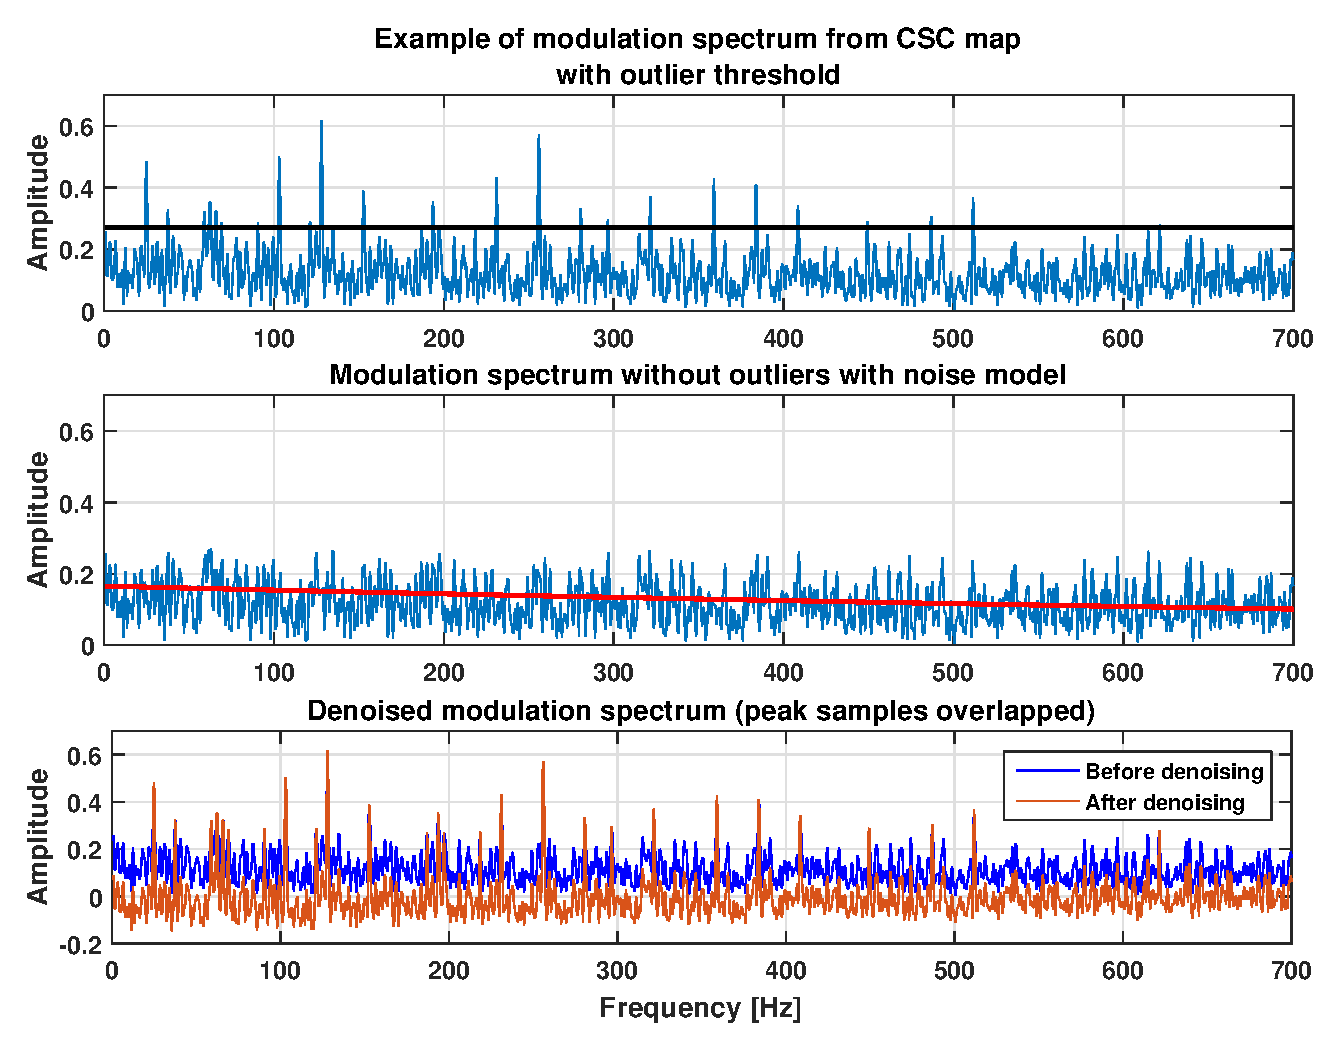
\includegraphics[width=.8\textwidth]{wykresy/ex}
\caption{Example of spatial denoising}
\label{fig:ex}
\end{figure}

% pokazać przykład że exp jest lepszy niż np linear i pokazac koniecznie R^2

\subsection{Monte Carlo simulation}\label{mcmc}

Monte Carlo (MC) methods are a class of algorithms that utilize random sampling in numerical computation problems. The main idea is to use large-scale randomness to discover deterministic behavior in the regarded problem. By the law of large numbers, the expected value of a random variable can be obtained approximately by averaging independent samples of the variable using i.e. mean, median etc. 

In presented application MC simulation is used to obtain good-quality envelope spectrum of damage component in the diagnostic signal. In practice, the role of random sampling is played by calculating randomly initialized NMF of denoised CSC map, using information provided by obtained encoding matrix, and based on that extracting envelope spectrum related to local damage. Such spectrum will not be exactly the same in every MC iteration, however, it is expected that most of the time outcome will be mostly correct. Finally, averaging of obtained results is expected to reveal true envelope spectrum related to damage by getting rid of uncommon frequency components.

Within the MC iterations, NMF is used to distinguish the predefined amount of groups $k$ of different behavior to be found in denoised CSC map. Those groups are here called classes. As mentioned before, one of them is expected to carry information about the informative component related to local damage. For the interpretation of obtained classes, authors take advantage of the encoding matrix operating in the domain of modulating frequency. It is easiest to visualize this operation as using posterior probability data (class indicator data) produced by a clustering algorithm. Encoding matrix can be interpreted as carrying information which class given point (here - given frequency component as entire spectrum vector in carrier domain integrated to a single value in modulation domain) belongs to. Using this information it is possible to construct envelope spectrum for each class. At this point, it is important to be able to automatically select cluster of interest. It is done by calculating kurtosis value (see section \ref{kurt}) of envelope spectrum vector for each class and selecting class with the highest value. It is motivated by the fact, that spectrum of this class is expected to contain a small number of different frequency components, with the majority of zero values, while other classes will be populated much more densely with frequency components carrying more coherent values of energy. In this context, kurtosis value is expected to be highest for the class related to damage.

Finally, the entire set of envelope spectra obtained from MC iterations has to be averaged to obtain the final result. Typically it is done using the ordinary sample mean, however in this application such approach would be disadvantageous. Due to random initialization of NMF, in most cases selected classes of envelope spectra are expected to contain a small number of improper frequency components in the notion of false-positive result or, on the other hand, to have expected correct frequency components missing. After using the sample mean to average large amount of obtained spectra, those impurities of the first type (false-positives) will remain as small values contaminating the desired perfect spectrum after averaging. To avoid this effect, authors used the median function for averaging the spectra. This way, unwanted contaminants will be omitted, instead of reduced.

As a summary of this section, single MC iteration is constructed as follows:

\begin{itemize}
    \item Factorize denoised CSC map with NMF;
    \item Use encoding matrix as indicator data to assign spectra vectors to their respective classes;
    \item Integrate spectra vectors within each class placing them at correct positions with respect to the modulating frequencies they stand for, which forms envelope spectra for all classes;
    \item Select class representing component of interest.
\end{itemize}

\subsubsection{Kurtosis as criterion for cluster selection}\label{kurt}

In the described application for every MC iteration, it is imperative to be able to automatically identify vector loosely populated with high-value nonuniform samples (highly non-Gaussian distribution) from among other vectors populated more densely with a larger amount of similar values (closer to Gaussian distribution). In such context it is a reasonable idea to select vector with the highest value of kurtosis, which is defined as follows:

\begin{equation}
\label{eq:kurtosis}
Kurt[X]=\frac{m_4}{{m_2}^2}=\frac{\frac{1}{n} \sum_{i=1}^{n} \left(x_i - \overline{x} \right)^4}{\left({\frac{1}{n} \sum_{i=1}^{n} \left(x_i - \overline{x} \right)^2}\right)^2}
\end{equation}
where $m_4$ is the fourth sample central moment and $m_2$ is the second sample central moment (sample variance).

\section{Application to real data}

In this section authors present the results of analysis of real-life industrial vibration data using described method. Figure~\ref{fig:csc} presents CSC map calculated from the input signal shown in Figure~\ref{fig:raw}. 

\begin{figure}[ht!]
\centering
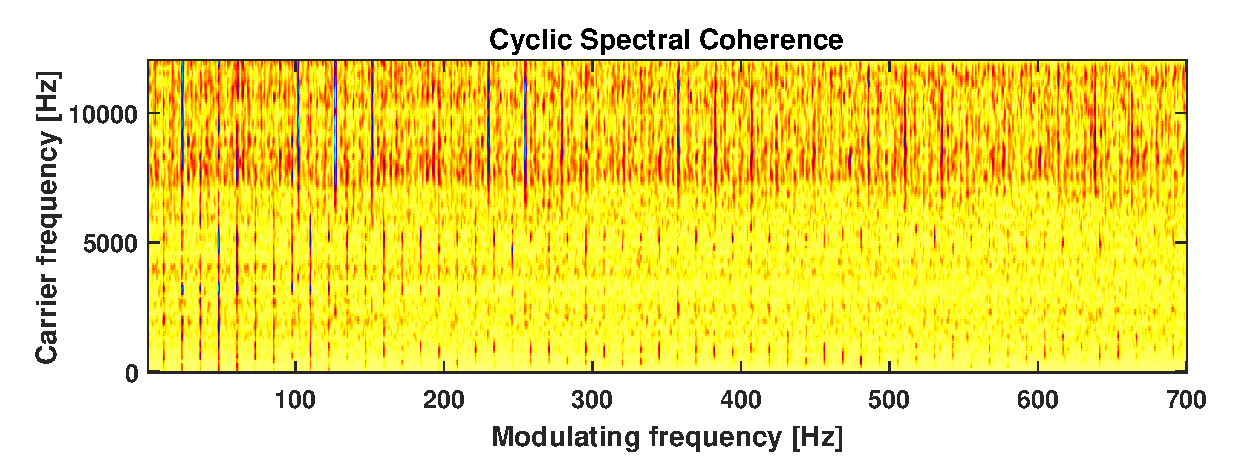
\includegraphics[width=.7\textwidth]{wykresy/csc}
\caption{Cyclic Spectral Coherence map for the first stage}
\label{fig:csc}
\end{figure}

After primary factorization with NMF algorithm set to 2 classes, authors takes advantage of base matrix that contains set of filters calculated for this particular CSC map. Figure~\ref{fig:trans} presents it on bottom left panel as a two-row matrix with carrier frequency axis common for filter bank and CSC map. On the right panels filters are drawn conventionally. 

\begin{figure}[ht!]
\centering
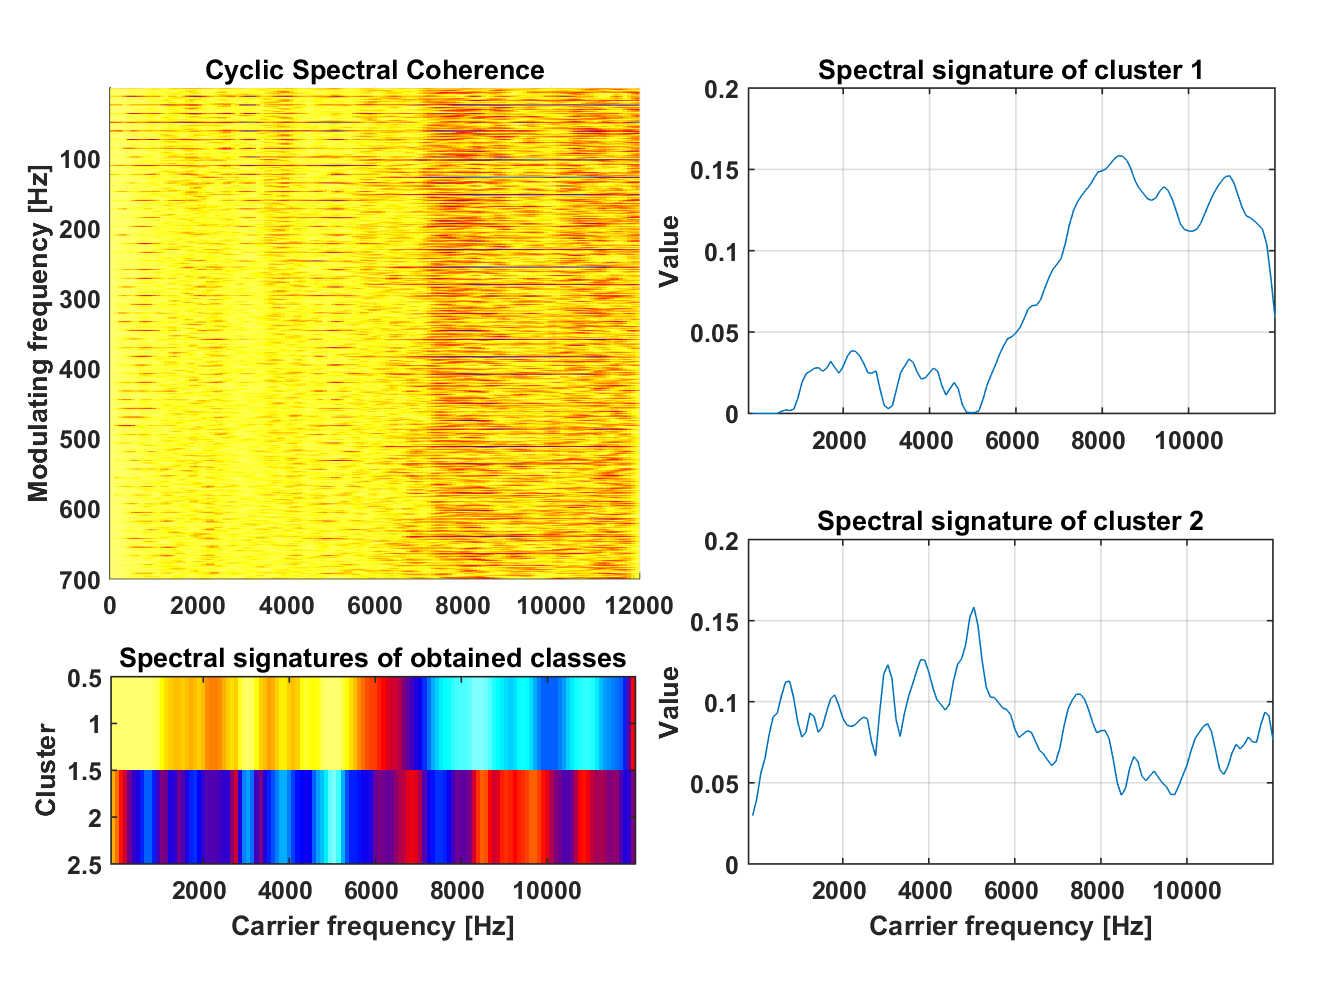
\includegraphics[width=.8\textwidth]{wykresy/trans}
\caption{Construction of filter bank using NMF base matrix}
\label{fig:trans}
\end{figure}

After that input signal is filtered with every filter from the bank (Figure~\ref{fig:out} left panels) and envelope spectra of obtained output signals are calculated for the evaluation of spectral structure (Figure~\ref{fig:out} right panels). Envelope spectrum of the second cluster contains fundamental frequency component of $12,35$ Hz and its harmonics that are the indicators of the rotational speed of the compressor shaft. On the other hand, the first cluster reveals the fundamental frequency of $127,9$ Hz and its harmonics, that additionally occur with very regular sidebands. Fundamental frequency perfectly corresponds with the expected frequency of BPFI for this bearing, while the presence of sidebands suggests the cyclic modulation in the signal that is also very common in cases of local damage in rotating elements. It is easy to conclude that this is the cluster of interest, but this information can be also obtained in an automatic way by finding a cluster with greatest SNR of the time series. Note that the change of scale in the time series for obtained clusters (scaling of vertical axis) occurs due to characteristic of the filter, that even in the passband takes the values less then one, however it does not affect the structure of the signal but only it's amplitude.

\begin{figure}[ht!]
\centering
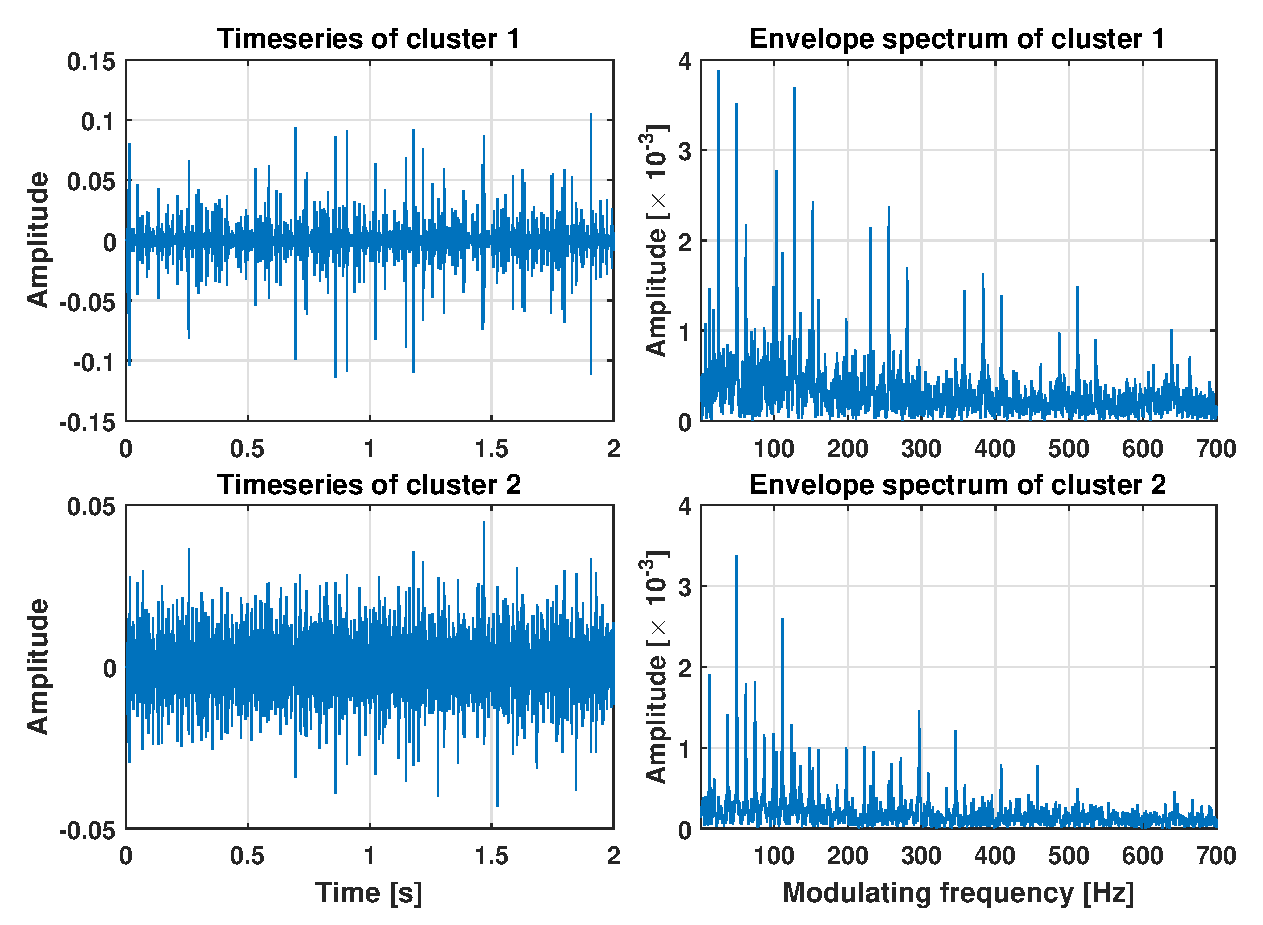
\includegraphics[width=.75\textwidth]{wykresy/out}
\caption{Results of method operation. Left panels: extracted time series, right panels: corresponding envelope spectra.}
\label{fig:out}
\end{figure}

While for experienced user it could be possible to identify the character of the damage already, envelope spectrum is still not very clean and a lot of different frequency components are present, especially within lower frequency bands and in terms of significant background noise. Hence, the second stage of presented methodology is expected to clean the signal by spatial denoising of CSC map.

\begin{figure}[ht!]
\centering
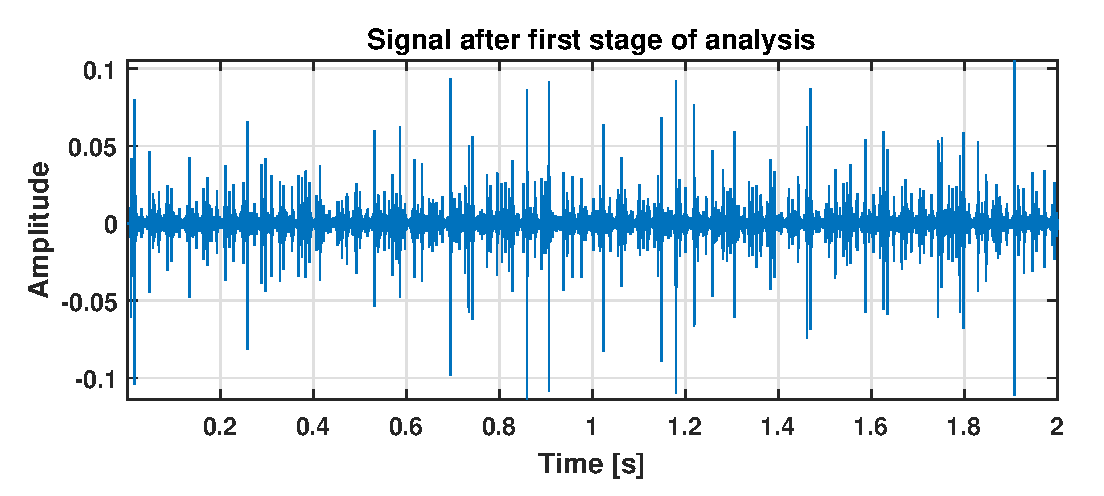
\includegraphics[width=.65\textwidth]{wykresy/raw2}
\caption{Input signal for the second stage}
\label{fig:raw2}
\end{figure}

Input signal for this stage (being the time series of first cluster from first stage of analysis, see Figure~\ref{fig:raw2}) is decomposed into CSC map of its own (see Figure~\ref{fig:csc2}). After that spatial noise model matrix is constructed according to description in section~\ref{denoise} (see Figure~\ref{fig:spd}) and subtracted from CSC map. This way it is possible to present and utilize new denoised CSC map, that is provided for the third stage of analysis (see Figure~\ref{fig:csc3}).

\begin{figure}[ht!]
\centering
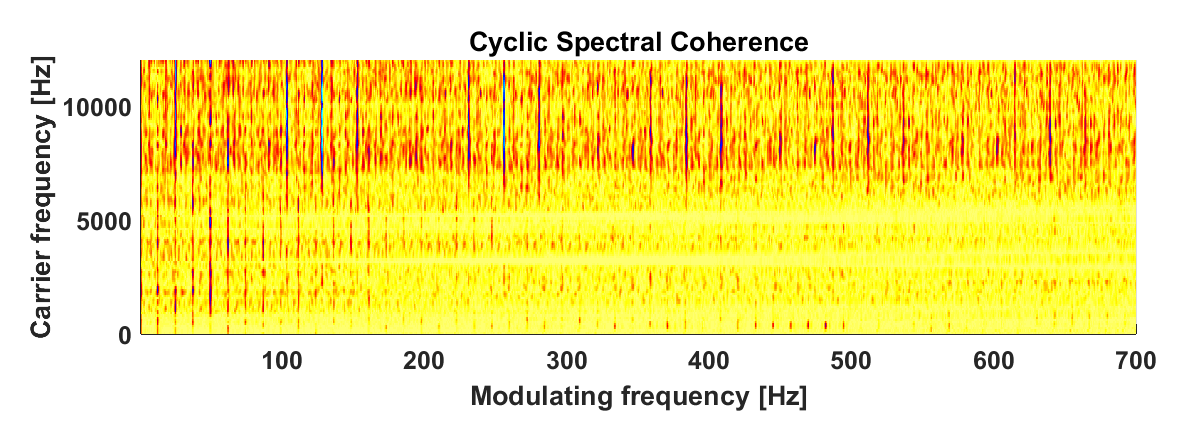
\includegraphics[width=.8\textwidth]{wykresy/csc2}
\caption{Cyclic Spectral Coherence map for the second stage}
\label{fig:csc2}
\end{figure}

\begin{figure}[ht!]
\centering
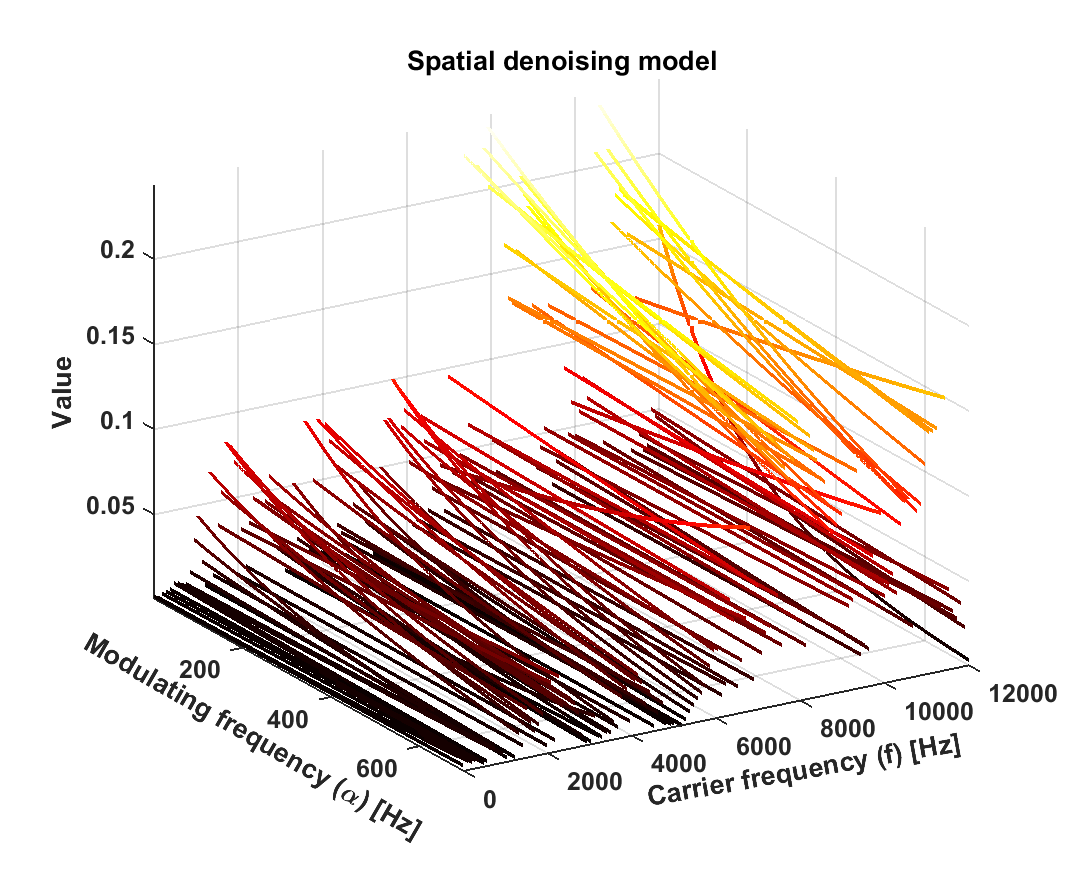
\includegraphics[width=.75\textwidth]{wykresy/spd}
\caption{Spatial denoising model}
\label{fig:spd}
\end{figure}

\begin{figure}[ht!]
\centering
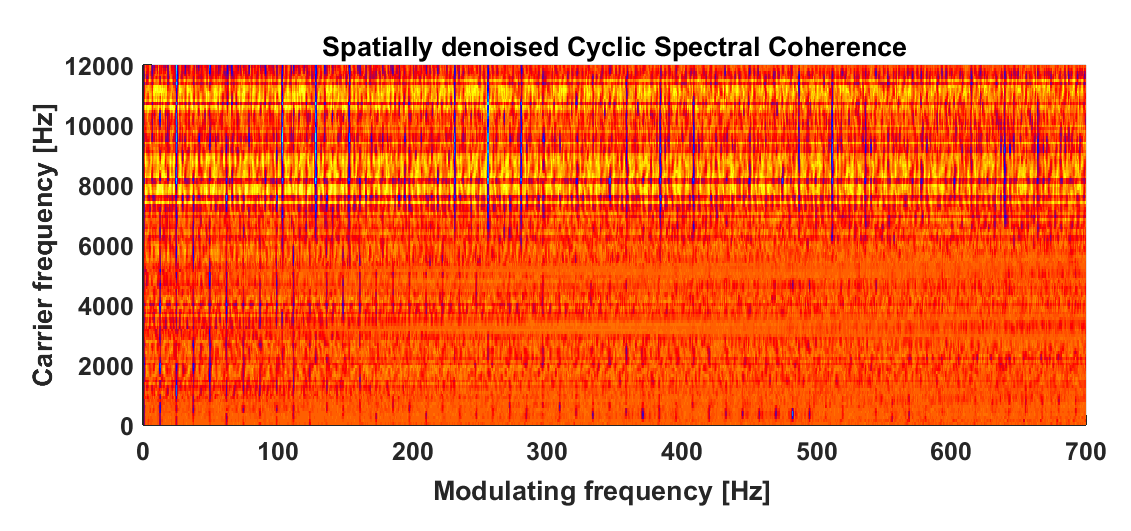
\includegraphics[width=.75\textwidth]{wykresy/csc3}
\caption{Spatially denoised Cyclic Spectral Coherence map}
\label{fig:csc3}
\end{figure}

At this point third stage of analysis begins, majority of which is focused on Monte Carlo iterations described in detail in section \ref{met}. For the purpose of robustness NMF factorization in this stage was set to six classes. \textcolor{red}{Figure \ref{fig:enc} presents the example of how classes might look like in a single MC iteration as an encoding matrix, and Figure \ref{fig:classes} presents them as individual plots. It is directly the encoding matrix of NMF, but its vectors are presented on individual plots. It is visible that top-center ($2^{nd}$) cluster contains spectrum related to shaft rotation and bottom-left ($4^{th}$) cluster stands for the damaged bearing signature.} However, it is clear that in this example spectra are not selected perfectly, which is very common effect, easiest observable on the damage cluster. Desired cluster describing damage spectrum is automatically selected with maximum value of kurtosis of spectrum vector. 
\begin{figure}[ht!]
\centering
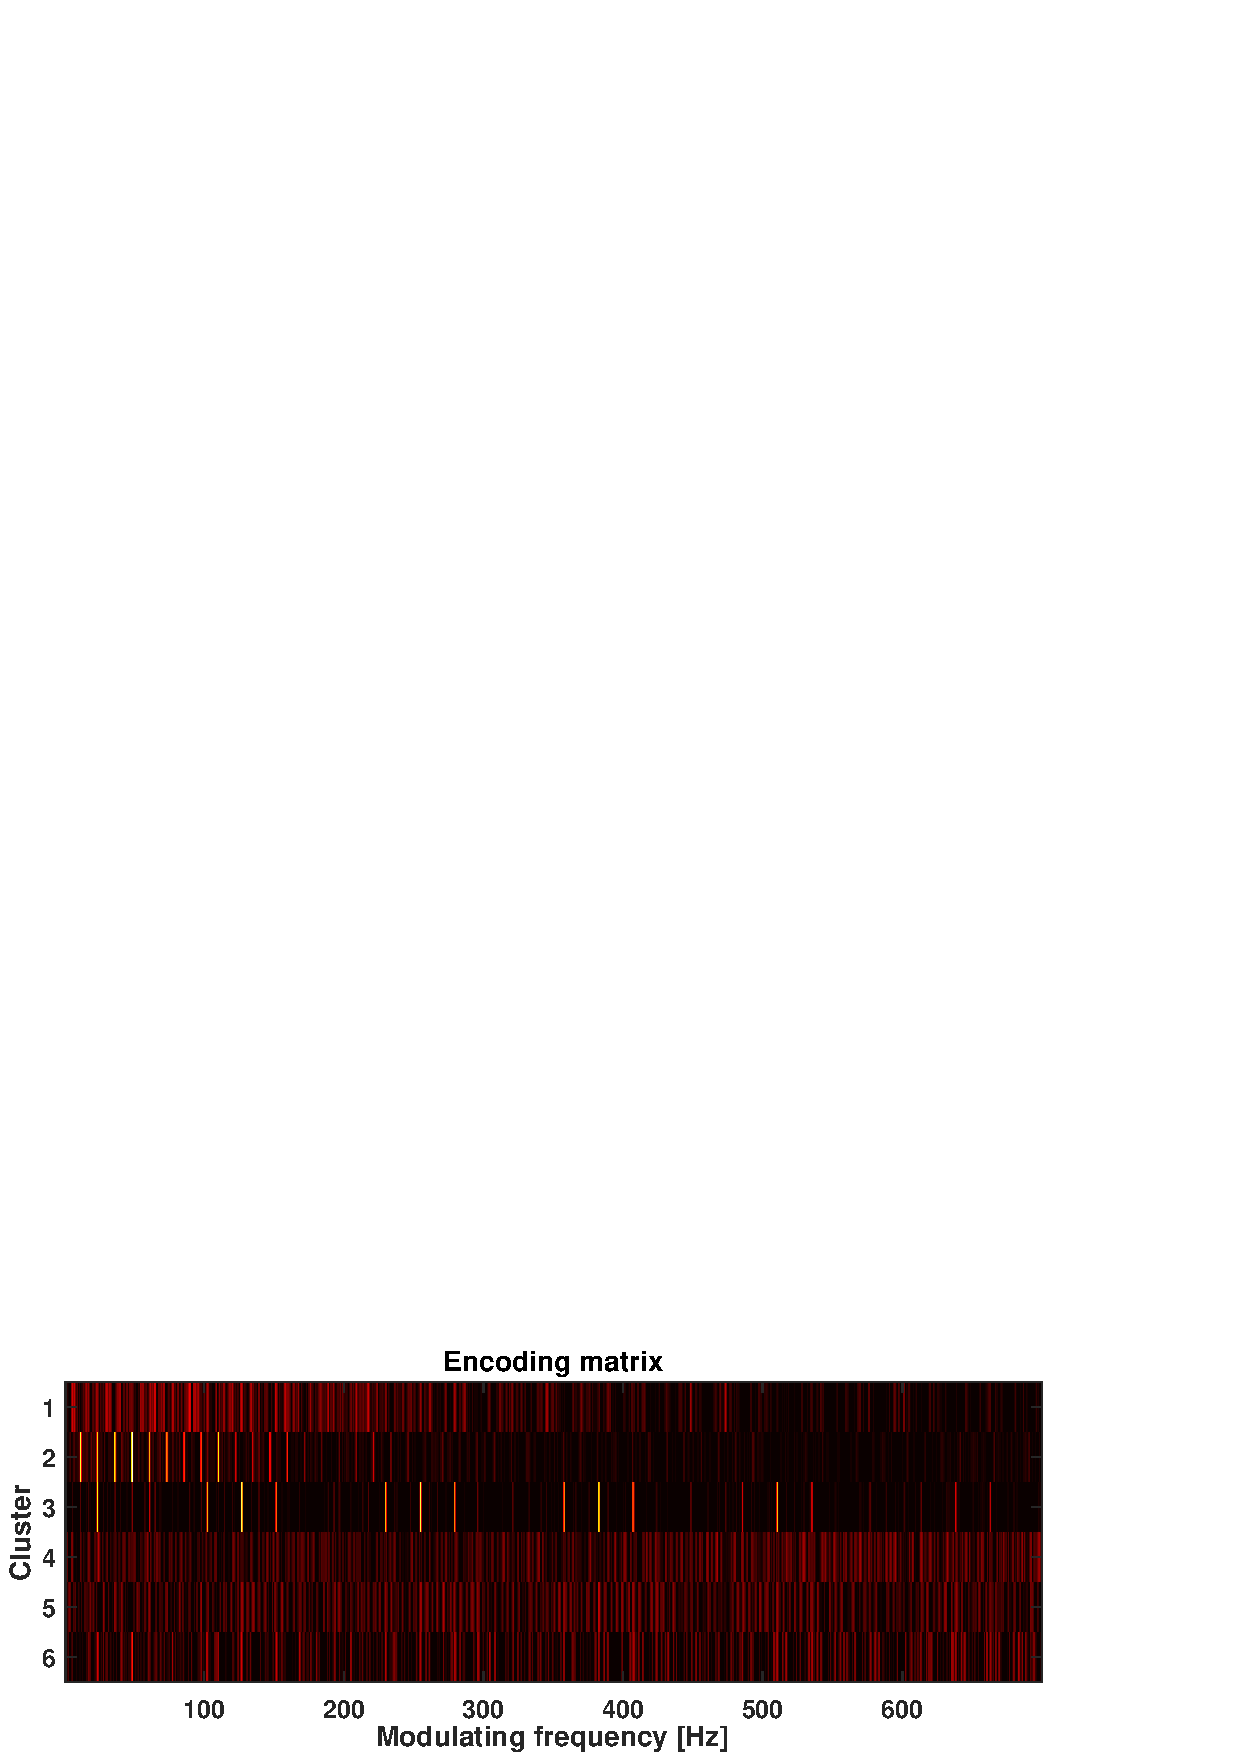
\includegraphics[width=.8\textwidth]{wykresy/enc2.png}
\caption{Example of encoding matrix produced by NMF in a single Monte Carlo iteration}
\label{fig:enc}
\end{figure}

\begin{figure}[ht!]
\centering
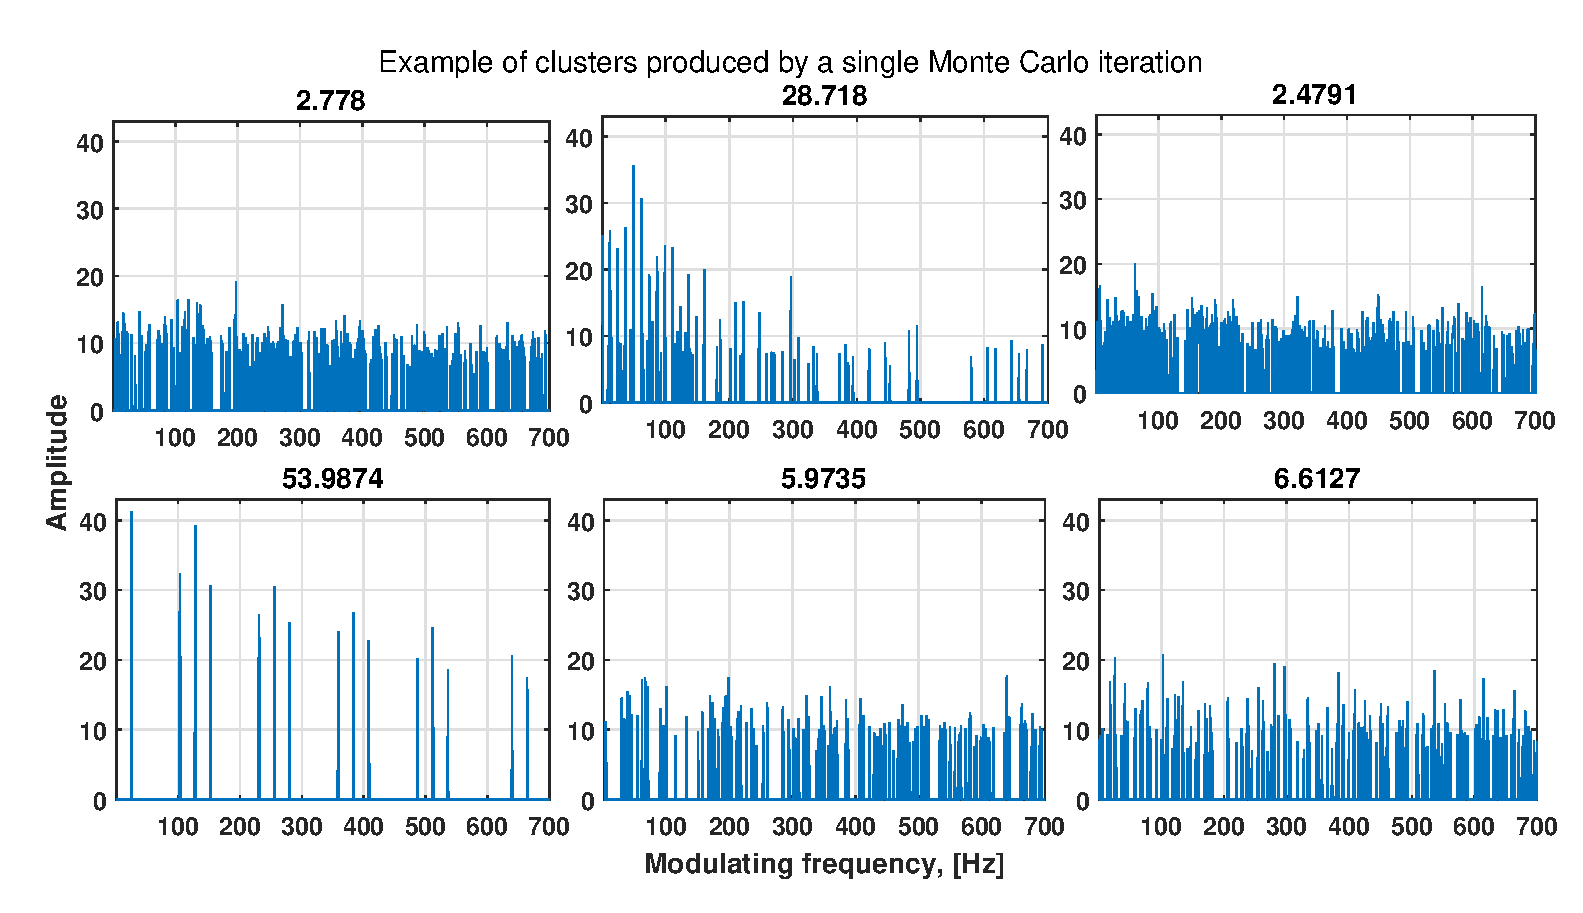
\includegraphics[width=.8\textwidth]{wykresy/clusters.eps}
\caption{Example classes produced by NMF in a single Monte Carlo iteration, numbers in panel titles indicate cluster kurtosis}
\label{fig:classes}
\end{figure}

\begin{figure}[ht!]
\centering
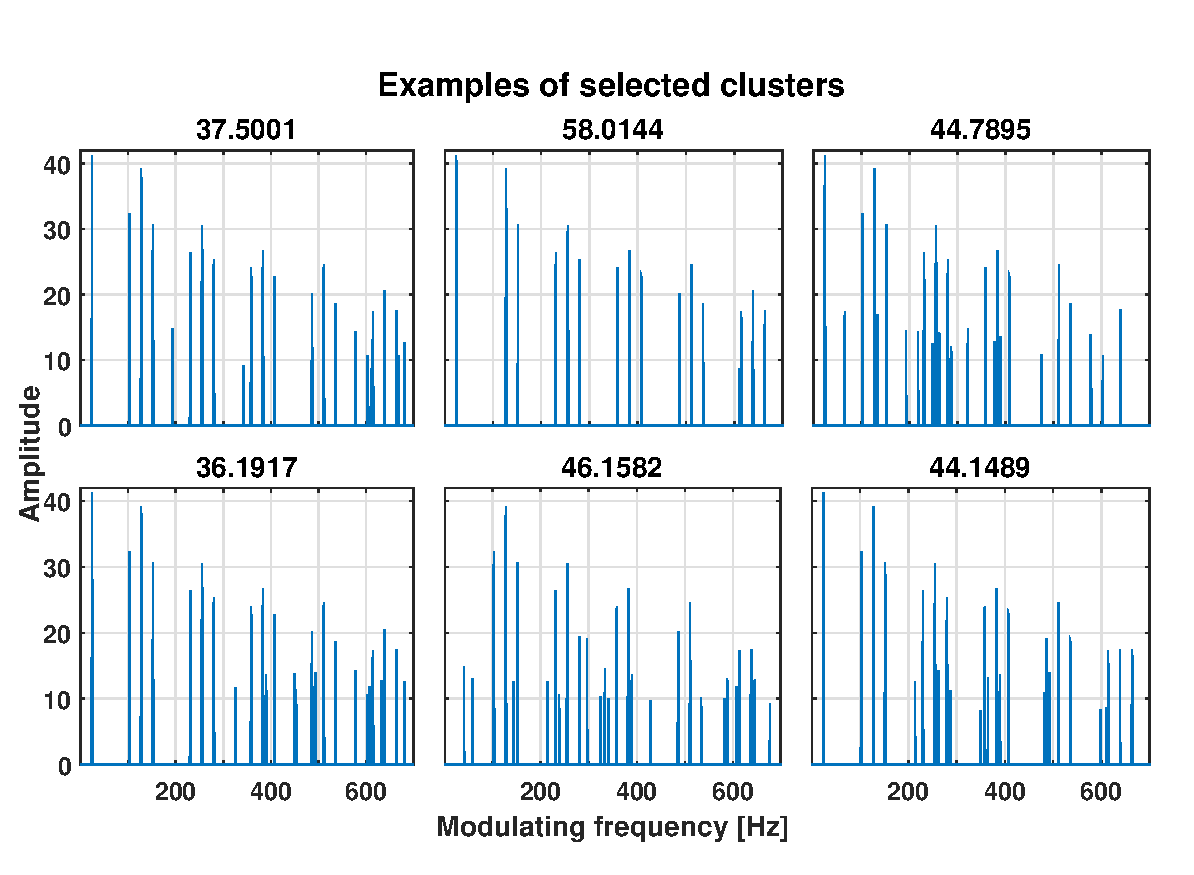
\includegraphics[width=.75\textwidth]{wykresy/multi.eps}
\caption{Examples of selected clusters}
\label{fig:multi}
\end{figure}

\textcolor{red}{Figure \ref{fig:multi} presents examples of damage cluster properly selected in consecutive MC iterations.} As explained before, those clusters will not be identical, but most of the time they are mostly correct, which is why MC technique is used to mitigate this effect. Finally median of selected clusters is calculated to extract common components. Envelope spectrum obtained that way is a perfect representation of frequency components related to damage (see Figure \ref{fig:out2}). Note that the amplitudes of components are much higher in comparison to the envelope spectra presented in earlier stages of the method. This effect occurs because of the fact that presented final envelope spectrum is in fact obtained by the sum of correlation coefficients across the CSC map. Hence, those summation can produce such high values. As it was stated before, the most important thing is to obtain clear pattern (fault frequencies surrounded by the sidebands with no additional noise floor).

\begin{figure}[ht!]
\centering
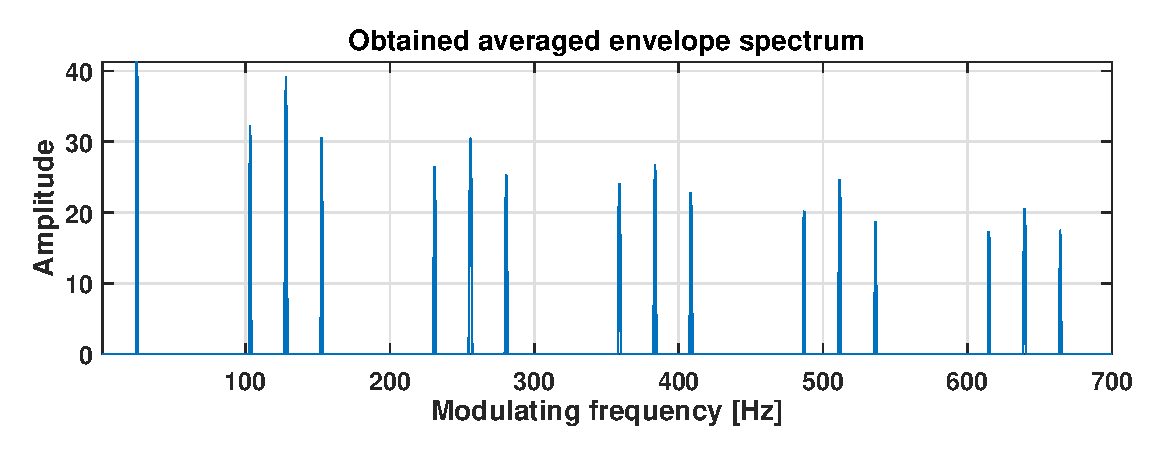
\includegraphics[width=.7\textwidth]{wykresy/out2}
\caption{Final damage component envelope spectrum}
\label{fig:out2}
\end{figure}

\section{Conclusions}

In this paper, authors have introduced a new method of local damage detection based on bi-frequency domain analysis, Nonnegative Matrix Factorization, spatial denoising and Monte Carlo simulation. The method is applied to the real vibration signals measured on the rolling bearing operating in an industrial gas compressor. The presented algorithm is especially suited for the cases when multiple cyclic impulsive components are present in the signal, which is very difficult to analyze using well-known classical methods. The proposed method is multi-stage and utilizes NMF from two different perspectives. First, it allows to initially separate cyclic components in carrier frequency domain, and then it is used as a tool for frequency components selection in the modulation domain. Additionally, spatial denoising stage helps to improve the quality of CSC map before the final stage of the algorithm. Monte Carlo simulation is used to decrease the undesired influence of randomness in NMF initialization. Application to real-life industrial data allows concluding that presented method can successfully unravel spectral signature of the fault in the investigated machine from amongst other impulsive components.

\section*{Bibliography}

% \bibliographystyle{JVE_style}
\bibliography{mybibfile}
\end{document}